%%%%%%%%%%%%%%%%%%%%%%%%%%%%%%%%%%%%%%%%%
% NIWeek 2014 Poster by T. Reveyrand
% www.microwave.fr
% http://www.microwave.fr/LaTeX.html
% ---------------------------------------
%
% Original template created by:
% Brian Amberg (baposter@brian-amberg.de)
%
% This template has been downloaded from:
% http://www.LaTeXTemplates.com
%
% License:
% CC BY-NC-SA 3.0 (http://creativecommons.org/licenses/by-nc-sa/3.0/)
%
%%%%%%%%%%%%%%%%%%%%%%%%%%%%%%%%%%%%%%%%%

%----------------------------------------------------------------------------------------
%   PACKAGES AND OTHER DOCUMENT CONFIGURATIONS
%----------------------------------------------------------------------------------------

\documentclass[a0paper,portrait]{baposter}

\usepackage[font=small,labelfont=bf]{caption} % Required for specifying captions to tables and figures
\usepackage{booktabs} % Horizontal rules in tables
\usepackage{relsize} % Used for making text smaller in some places

\usepackage{amsmath,amsfonts,amssymb,amsthm} % Math packages
\usepackage{eqparbox}

\usepackage{textcomp}

\usepackage{caption}
\usepackage{subcaption}
\usepackage{graphicx}
\usepackage{listings}
\usepackage{mathtools}
\usepackage[percent]{overpic}


\usepackage{multirow}
%\usepackage{verbatimbox}
%\usepackage{hyperref}

%\usepackage{pgf}

\usepackage[utf8]{inputenc}
\usetikzlibrary{shapes,arrows}
\usepackage{tikz}
\usetikzlibrary{automata,positioning}

\usepackage{multicol}

\usepackage{hyperref}

\usepackage[font=small,labelfont=bf]{caption}

\usepackage{makecell}
\usepackage{enumitem}

\renewcommand\theadalign{bc}
\renewcommand\theadfont{\bfseries}
\renewcommand\theadgape{\Gape[4pt]}
\renewcommand\cellgape{\Gape[4pt]}


\setlist[itemize]{leftmargin=*}

\graphicspath{{figures/}} % Directory in which figures are stored

 \definecolor{bordercol}{RGB}{40,40,40} % Border color of content boxes
 \definecolor{headercol1}{RGB}{210,235,250} % Background color for the header in the content boxes (left side)
 \definecolor{headercol2}{RGB}{210,235,250} % Background color for the header in the content boxes (right side)
 \definecolor{headerfontcol}{RGB}{0,0,0} % Text color for the header text in the content boxes
 \definecolor{boxcolor}{RGB}{240,255,255} % Background color for the content in the content boxes

\tikzset{
    state/.style={
           ellipse,
           draw=black, thin,
           minimum height=0.5cm,
           minimum width=0.6cm,
           text centered,
           font=\scriptsize
           },
    horiz/.style={
           % font=\tiny,
           inner sep=3pt,
           font=\bf

           } ,
    point/.style={
           circle,
           minimum width = 5pt,
           fill
           }
}

\begin{document}

\setlength{\fboxsep}{0pt}

\background{ % Set the background to an image (background.pdf)
\begin{tikzpicture}[remember picture,overlay]
\draw (current page.north west)+(-2em,2em) node[anchor=north west]
{
\includegraphics[height=1.1\textheight]{background}};
\end{tikzpicture}
}

\begin{poster}{
grid=false,
columns=12, % because reasons
borderColor=bordercol, % Border color of content boxes
headerColorOne=headercol1, % Background color for the header in the content boxes (left side)
headerColorTwo=headercol2, % Background color for the header in the content boxes (right side)
headerFontColor=headerfontcol, % Text color for the header text in the content boxes
boxColorOne=boxcolor, % Background color for the content in the content boxes
headershape=rectangle, % Specify the rounded corner in the content box headers
headerfont=\Large\sf\bf, % Font modifiers for the text in the content box headers
textborder=none,
background=none,
headerborder=none, % Change to closed for a line under the content box headers
boxshade=plain
}
{
\includegraphics[width=4cm]{jr.png}}
%
%----------------------------------------------------------------------------------------
%   TITLE AND AUTHOR NAME
%----------------------------------------------------------------------------------------
%
{\bf \huge{Context-Free Path Querying with Single-Path Semantics by Matrix Multiplication} }
%\\  \Large \it Context-free grammars and neural networks for secondary structure} % Poster title
{\vspace{0.6em} \smaller \textbf{Rustam Azimov} \\  % Author names
\smaller \it {JetBrains Research, Saint Petersburg University, Russia } \\ % Author email addresses
\smaller  {Rustam.Azimov@jetbrains.com}}
{
\includegraphics[width=2.5cm]{SPbGU_Logo.png}} % University/lab logo


%----------------------------------------------------------------------------------------
%   INTRODUCTION
%----------------------------------------------------------------------------------------
\begin{posterbox}[name=CFPQ,column=0,row=0, span=4]{Relational CFPQ}

  Find paths which satisfy constraints in form of a formal language $L=\{a^n b^n \mid n > 0\}$
    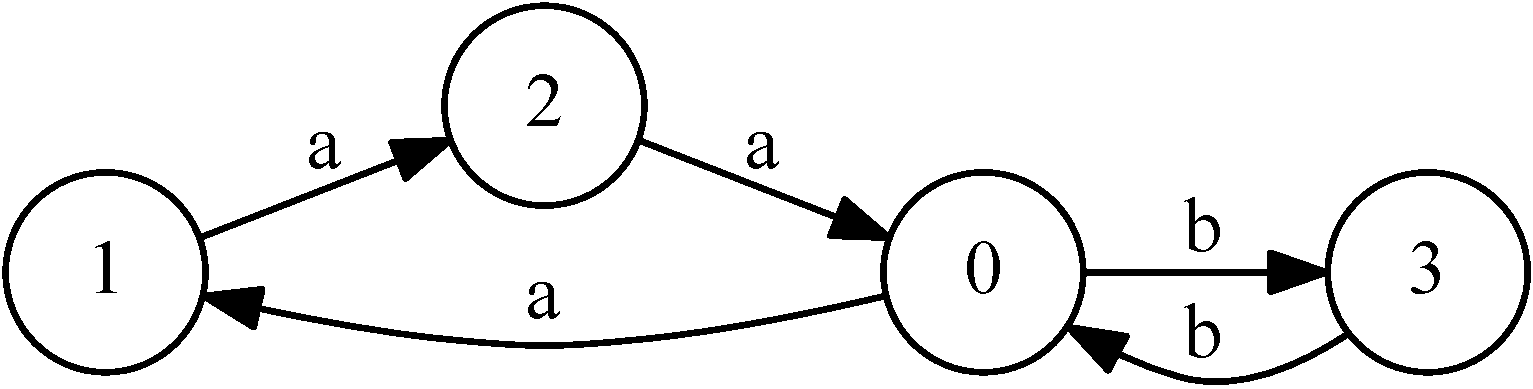
\includegraphics[width=7cm]{example_graph_transparent.png}

    Query = grammar for $L$: $S  \rightarrow a  \ b \ | \ a \ S \ b  \\$

  Result: $ \{(u,v) \mid \exists p \text{ from } u \text{ to } v: \text{word}(p) \in L\} $

\end{posterbox}

\headerbox {Matrix-Based Algorithm~\cite{Azimov:2018:CPQ:3210259.3210264}}
{name=matrices,column=0,span=6, row=2, below=CFPQ}%,bottomaligned=sol2}
{

$T$ is an adjacency matrix of the input graph\\
The grammar is in the normal form
\vspace{-0.5cm}

\begin{align*}
T_{ij} &=\{ N \mid N \xRightarrow[]{*} \omega,  \omega \text{ -- path bw } i \text{ and } j \} \\
T_{ik} \times T_{kj} &= \{ A \mid B \in T_{ik}, C \in T_{kj}, A \rightarrow B C \} \\
T^{(i)} &= T^{(i-1)} \cup (T^{(i-1)} \times T^{(i-1)})
\end{align*}

\begin{itemize}
  \item Can be formulated in terms of boolean matrices multiplication
  \item Easy to run in parallel environments: GPUs, multithreaded CPUs, clusters
%  \item Existing matrix multiplication library can be used
\end{itemize}
\vspace{0.1cm}
}

\headerbox {Results}{name=results,column=4,row=0, span=4, bottomaligned=CFPQ}{
\begin{itemize}
  \item We provide the matrix-based algorithm for CFPQ with single-path query semantics
  \item We provide several implementations of the CFPQ algorithms for both query semantics which use RedisGraph as graph storage
  \item We extend the dataset presented in~\cite{Mishin:2019:ECP:3327964.3328503} with new real-world and synthetic cases of CFPQ
\end{itemize}
}

\headerbox {Future Research}{name=answers,column=8,row=0, span=4, bottomaligned=results}{

\begin{itemize}
  \item Extend the matrix-based CFPQ algorithm to all-path
  query semantics
  \item Update the query results dynamically when data changes
  \item Include real-world cases from
  the area of static code analysis to the dataset
  \item Find new applications that required CFPQ
\end{itemize}

}


\headerbox {CFPQ with Single-Path Semantics}
{name=impl,column=6,span=6, row=2, below=results,bottomaligned=matrices}
{
\begin{itemize}
	\item We also need to provide one such path for all node pairs $(u,v)$
	\item Use $\textit{PathIndex} = (\textit{left},\textit{right},\textit{middle},\textit{height},\textit{length})$ as matrix elements
	\begin{itemize}
		\item $left$, $right$ --- the starting and the ending node of the path
		\item $middle$ --- the intermediate node of last path concatenation
		\item $\textit{height}$, $\textit{length}$ --- the height and the length of path			
	\end{itemize}
    \item Update the matrix operations to keep PathIndexes correct
    \item After the CFPQ algorithm we can extract the path stored
    \item The path extraction time is small and linear in the length of the path
\end{itemize}
}

\setlength{\tabcolsep}{5pt}
\headerbox{New Implementations of CFPQ}{name=rdfs,span=12,column=0,row=3,below=matrices}{
	\vspace{0.05cm}
	\begin{minipage}[t]{0.48\textwidth}
		\begin{itemize}
			\item We use RedisGraph graph database as storage
			\item CPU-based implementations:
			\begin{itemize}
				\item $\textbf{RG\_CPU}_{\textit{rel}}$ --- for the relation query semantics			
				\item $\textbf{RG\_CPU}_{\textit{path}}$ --- for the single-path query semantics			
			\end{itemize}
		\end{itemize}
	\end{minipage}
	~
	\begin{minipage}[t]{0.5\textwidth}
		\begin{itemize}
			\item GPGPU-based implementations:
			\begin{itemize}
				\item $\textbf{RG\_CUSP}_{\textit{rel}}$ --- relational semantics, utilizes a \textbf{CUSP} library
				
				\item $\textbf{RG\_GPU}_{\textit{rel}}$ --- relational semantics, uses low-latency on-chip shared memory for the hash table of each row of the result matrix
				
				\item $\textbf{RG\_GPU}_{\textit{path}}$ --- single-path semantics, operating over PathIndex
			\end{itemize}
		\end{itemize}
	\end{minipage}
}


\headerbox{CFPQ Evaluation with Relational and Single-Path Query Semantics}{name=scaling,span=12,column=0,row=2,below=rdfs}{
\vspace{0.05cm}
%\begin{table}[h]
%\rowcolors{1}{}{red}
%\begin{center}
\begin{minipage}[t]{0.7\textwidth}
%\vspace{-4.5cm}
\begin{tabular}{| l | c | c | r  r | r  r | r  r | r  r |}
	\hline
	
	\multirow{3}{*}{Name} & \multirow{3}{*}{\#V} & \multirow{3}{*}{\#E}  &   \multicolumn{4}{|c|}{Relational semantics index}	&	\multicolumn{4}{|c|}{Single path semantics index} \\
	\cline{4-11} & &
	&	\multicolumn{2}{|c|}{RG\_CPU\textsubscript{rel}}	&	\multicolumn{2}{|c|}{RG\_GPU\textsubscript{rel}} &	\multicolumn{2}{|c|}{RG\_CPU\textsubscript{path}}	&	\multicolumn{2}{|c|}{RG\_GPU\textsubscript{path}}	 \\
	\cline{4-11} & &
	&   Time & Mem &  Time     & Mem & Time     & Mem   & Time     & Mem \\
	\hline
	\hline
	%core           & 1,323		& 8,684              & 0.004 & 0.3    & 0.010  & 0.1      & 0.002 & 0.3  & 0.016 & 0.1  \\
	pathways        & 6,238		& 37,196           & 0.011 & 0.1    & 0.007 & 0.1      & 0.021 & 0.5  & 0.021 & 2.0    \\
	go-hierarchy    & 45,007	& 1,960,436        & 0.091 & 16.3    & 0.108 & 121.2    & 0.976 & 92.0   & 0.336 & 125.0  \\
	enzyme          & 48,815	& 219,390          & 0.018 & 5.9     & 0.018 & 4.0        & 0.029 & 8.1  & 0.043 & 6.0    \\
	eclass\_514en   & 239,111	& 1,047,454        & 0.067 & 13.8     & 0.166 & 16.0     & 0.195 & 31.2 & 0.496 & 26.0   \\
	
	
	go              & 272,770	& 1,068,622        & 0.604 & 28.8     & 0.365 & 30.2     & 1.286 & 75.7 & 0.739 & 45.4 \\
		
	geospecies      & 450,609	& 4,622,922        & 7.146 & 16934.2 & 0.856 & 5274 & 15.134 & 35803.6 & 1.935 & 5282   \\
	\hline
\end{tabular}
\end{minipage}~
\begin{minipage}[t]{0.3\textwidth}
\vspace{-2.2cm}
\begin{overpic}[width=0.98\textwidth]{plots/G1_go.pdf}
    \put (20,55) {{Path extraction time for \textbf{Go}}}
  \end{overpic}
%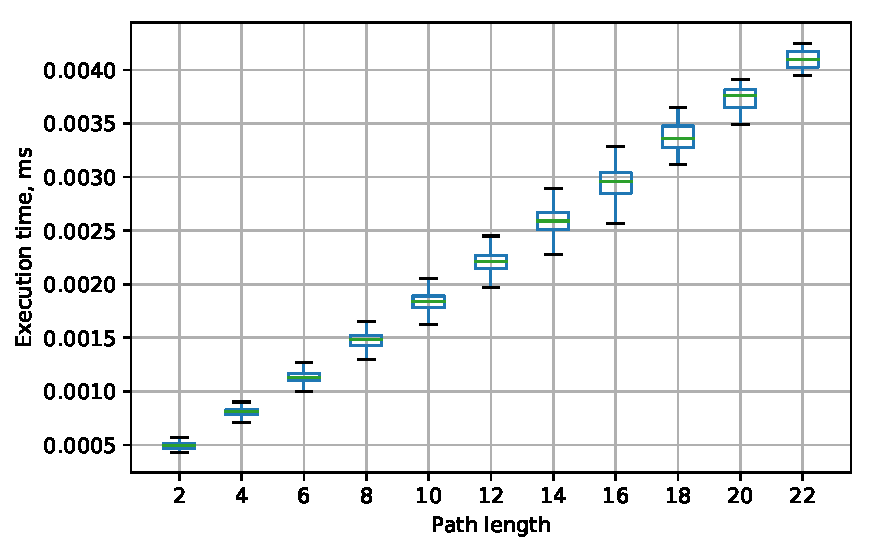
\includegraphics[width=0.95\textwidth]{plots/G1_go.pdf}
\end{minipage}

\begin{minipage}[t]{0.5\textwidth}
	\vspace{0.05cm}
	\begin{itemize}
		\item Time in seconds and memory is measured in megabytes
		\item  Graph: real-world ontologies (RDFs), query: same-generation query
		\item Example of a grammar: $S \to \textit{scor} \ S \ \textit{sco} \ | \ \textit{tr} \ S \ \textit{t} \ | \ \textit{scor} \ \textit{sco} \ | \ \textit{tr} \ \textit{t}$
	\end{itemize}
\end{minipage}
~
\begin{minipage}[t]{0.48\textwidth}
\vspace{0.05cm}
  \begin{itemize}
  	\item GPGPUs utilization significantly increases the performance
  	\item Implementations with sparse matrices significantly faster than others
  	\item The cost of computing matrices with PathIndexes is not high
  \end{itemize}
\end{minipage}
}



\headerbox {\smaller{Contact Us}}{name=contact,column=0,span=5,below=scaling}{
\scriptsize
\begin{minipage}[t]{0.65\textwidth}
  \vspace{-2.5cm}
\begin{itemize}
  \item Semyon Grigorev: \href{mailto:s.v.grigoriev@spbu.ru}{s.v.grigoriev@spbu.ru}
  \item Rustam Azimov:\href{mailto:Rustam.Azimov@jetbrains.com}{Rustam.Azimov@jetbrains.com}
  \item Arseniy Terekhov: \href{mailto:simpletondl@yandex.ru}{simpletondl@yandex.ru}
  \item Artyom Khoroshev: \href{mailto:arthoroshev@gmail.com}{arthoroshev@gmail.com}
\end{itemize}


\end{minipage}
~
\begin{minipage}[t]{3cm}

\includegraphics[width=2.8cm]{qr-research-jetbra.pdf}
\vspace{0.7cm}
\end{minipage}
%\vspace{1cm}
{\scriptsize
%Both dataset and implementations are available on GitHub
\vspace{-1cm}
\begin{itemize}
	\item Dataset link:
	\url{https://github.com/JetBrains-Research/CFPQ_Data}
	\item Implementations link:
	\url{https://github.com/YaccConstructor/RedisGraph}
\end{itemize}
}

}



\headerbox{\smaller{References}}{name=references,column=5,span=7,below=scaling}{

    \scriptsize % Reduce the font size in this block
    \renewcommand{\section}[2]{\vskip 0.05em} % Get rid of the default "References" section title
    \nocite{*} % Insert publications even if they are not cited in the poster
    \bibliographystyle{unsrt}
    \bibliographystyle{IEEEtran}
    \bibliography{biblio} % Use biblio.bib as the bibliography file
}

\headerbox {\smaller{Acknowledgments}}{name=ack,column=5,span=7,below=references}{
\small
The reported study was funded by grant from JetBrains Research and by RFBR, project number 19-37-90101
}

{\hspace{5pt}
\includegraphics[width=0.4\textwidth]{2020Sigmod-LOGO.png}}


\end{poster}


\end{document}
